% ------------------------------------
\section{Overview}
% ------------------------------------
\begin{frame}[fragile]{Frama-C Historical Context}
\begin{itemize}
\item 90's: \blue{CAVEAT}, Hoare logic-based tool for C code at CEA

\item 2000's: \blue{CAVEAT used by Airbus} during certification process of
  the A380 \gray{(DO-178 level A qualification)}

  \pause

\item 2002: \blue{Why} and its C front-end \blue{Caduceus} (at INRIA)
  
\item 2004: start of Frama-C project as a successor to CAVEAT and
  Caduceus

  \pause

  
\item 2008: \blue{First public release} of Frama-C \gray{(Hydrogen)}

\item {2012:  \blue{WP}: Weakest-precondition based plugin}

\item {2012: \blue{E-ACSL}: Runtime Verification plugin}

  \pause
  
\item {2013: CEA Spin-off \blue{TrustInSoft}}

  \pause
  
\item 2016: \blue{Eva}: Evolved Value Analysis

\item 2016: \blue{Frama-Clang}: C++ extension

\item 2017: \blue{Frama-C Sulfur} \gray{(v.16)}

\item Today: \blue{Frama-C Chlorine} \gray{(v.17)}
\end{itemize}
\end{frame}
%------------------------------------
\begin{frame}[fragile]{Frama-C Open-Source Distribution}

\begin{center}
  \large{\blue{Framework for Analysis of source code written in \gray{ISO 99}
      C}}
  
  {\small {\gray{[Kirchner et al, FAC'15]}}}
\end{center}
\vspace{-1mm}

\begin{itemize}
\item analysis of C code extended with \blue{ACSL} annotations
\smallskip
\item ACSL Specification Language
  \begin{itemize}
%  \item ISO/ANSI C Specification Language
  \item {\it langua franca} of Frama-C analyzers
  \end{itemize}
%\item developed by CEA LIST since 2005
%\smallskip
\item \gray{mostly} \blue{open-source} \gray{(LGPL 2.1)}
%% \smallskip
%% \item first open-source release \gris{aka Hydrogen} in 2008 
%% \smallskip
%% \item last open-source release \gris{aka Magnesium} in 2016/01
%% \smallskip
%% \item next open-source release \gris{aka Aluminium} expected in 2016/05\\
%\vspace{1pt}
%\smallskip
\begin{center}
  \large{\red{http://frama-c.com}}
\end{center}
\smallskip
\item also proprietary extensions and distributions
\smallskip
\item targets both \blue{academic} and \blue{industrial} usage
\end{itemize}


  \begin{center}
    \hfill
    
\includegraphics[scale=0.12]{logos/airbus.jpg}
    \hfill
    
\includegraphics[scale=0.12]{logos/atos.png}
    \hfill
    
\includegraphics[scale=0.12]{logos/edf.png}
    \hfill
    
\includegraphics[scale=0.12]{logos/areva.png}
    \hfill
    
\includegraphics[scale=0.12]{logos/irsn.png}\\
    \hfill
    
\includegraphics[scale=0.12]{logos/bv.png}
    \hfill
    
\includegraphics[scale=0.12]{logos/trustinsoft.png}
    \hfill
    
\includegraphics[scale=0.12]{logos/dassault.png}
    \hfill
    
\includegraphics[scale=0.12]{logos/mitsu.png}
    \hfill
  \end{center}

\end{frame}


%------------------------------------
\begin{frame}[label=exProven,fragile]{Example: a C Program Annotated in ACSL}
\lstinputlisting[language=C,alsolanguage=ACSL,basicstyle={\scriptsize}]{all_zeros_proved.c}
\raisebox{0mm}[0mm][0mm]{
  \begin{tikzpicture}
    \draw[fill,green] (1,1) circle (0pt);
    \node[markplace={(8,3)},below right=0.5cm and 1cm] {\begin{tabular}{c}Can be proven \\ with Frama-C/WP \end{tabular}};
  \end{tikzpicture}
}
\end{frame}

%%%%%%%%%%%%%%%%%%%%%%%%%%%%%%%%%%%%%%%%%%%%%%%%%%%%%%%%%%%%%%%%%%%%%%%%%%%%%%%

\begin{frame}{Frama-C, a Collection of Tools}

  \begin{center}
    \large{\red{Several tools inside a single platform}}
  \end{center}

\begin{itemize}
\item \blue{plugin architecture} like in Eclipse
  %{\small{\gray{[S. @F-IDE'15]}}}
\medskip
\item tools provided as plugins
  \smallskip
  \begin{itemize}
  \item over 20 plugins in the open-source distribution
  \smallskip
%  \item outside open-source plugins \gray{(E-ACSL \& Frama-Clang, a few
%    others)}
  \smallskip
  \item close-source plugins, either at CEA \gray{(about 20)} or outside
  \end{itemize}
\medskip
\item a common \blue{kernel}
  \smallskip
  \begin{itemize}
  \item provides a uniform setting
  \smallskip
  \item provides general services
  \smallskip
  \item synthesizes useful information
  \end{itemize}
\end{itemize}

\end{frame}

%------------------------------------

\begin{frame}{Plugin Gallery}

\vspace{-10mm}
\begin{center}
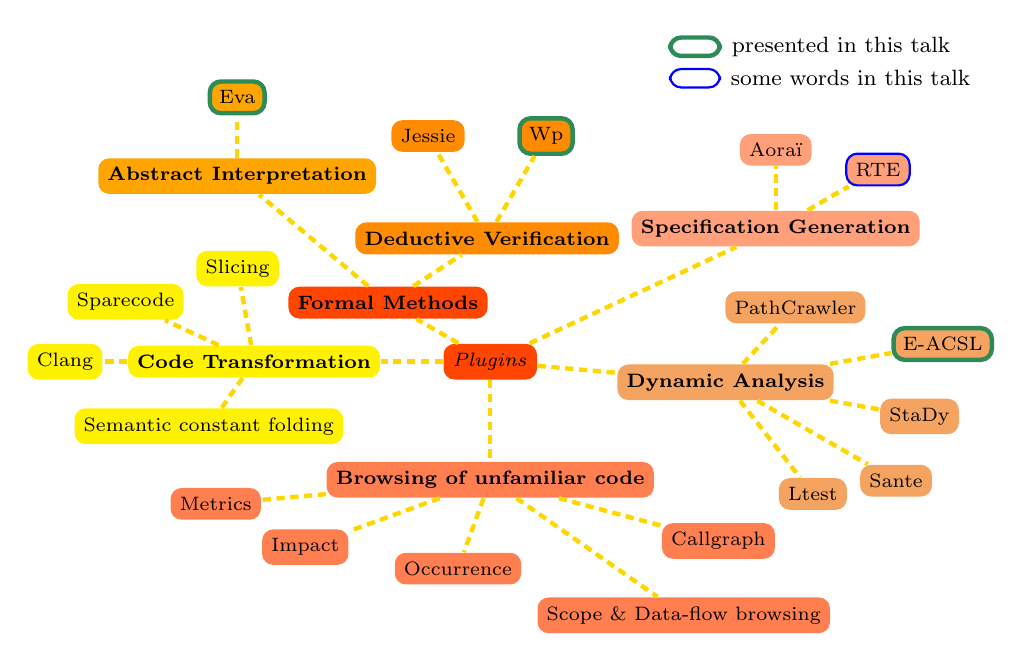
\begin{tikzpicture}[
  x=1mm,y=1mm,
  concept/.style={rectangle, rounded corners,font=\scriptsize, 
                        minimum height=0mm},
  edge from parent path={[draw,ultra thick, densely dashed, Gold](\tikzparentnode\tikzparentanchor) -- (\tikzchildnode\tikzchildanchor)
},
 presented/.style={draw=SeaGreen, ultra thick, solid},
 talking/.style={draw=blue, thick, solid}
  ]
\node[concept,presented, minimum width=18,minimum height=3,
      label=0:{\footnotesize presented in this talk},
      label distance = 5
] at (26,40) {};
\node[concept,talking, minimum width=18,minimum height=3,
      label=0:{\footnotesize some words in this talk},
      label distance = 5
] at (26,36) {};
\node[concept,fill=OrangeRed] {\textit{Plugins}}
  child[grow=-5 clockwise, concept/.append style={fill=SandyBrown}, 
    level distance=30mm]
  % Dynamic Analysis
  {node[concept] {\textbf{Dynamic Analysis}}
    child[grow=47 clockwise, level distance=13mm]
    {node[concept] {PathCrawler}}
    child[grow=10 clockwise, level distance=28mm]
    {node[concept,presented] {E-ACSL}}
    child[grow=-10 clockwise, level distance=25mm]
    {node[concept] {StaDy}}
    child[grow=-30 clockwise, level distance=25mm]
    {node[concept] {Sante}}
    child[grow=-52 clockwise, level distance=18mm]
    {node[concept] {Ltest}}
  }
  %%child[grow=20 clockwise, concept/.append, level distance=35mm]
  % Concurrency
  %% {node [concept] {Concurrency}
  %%   child[grow=20 clockwise, level distance=25mm]
  %%   {node[concept] {Mthread}}}
  % Specification Generation
  child[grow=25 clockwise, concept/.append style={fill=LightSalmon}, level
    distance=40mm ]
  {node[concept] {\textbf{Specification Generation}}
     %% child[grow=30 clockwise,level distance=15mm] 
     %%      {node[concept]{Agen}}
     child[grow=30 clockwise,level distance=15mm] 
          {node[concept,talking]{RTE}}
     child[grow=90 clockwise,level distance=10mm] 
          {node[concept]{Aoraï}}}
  child[grow=150 clockwise,, concept/.append style={fill=OrangeRed}]
  % Formal Methods
  {node[concept] {\textbf{Formal Methods}}
     child[grow=33 clockwise,
           level distance=15mm, concept/.append style={fill=DarkOrange}]
     % Deductive verification
     {node[concept]{\textbf{Deductive Verification}}
        child[grow=60 clockwise]{node[concept,presented]{Wp}}
        child[grow=120 clockwise]{node[concept]{Jessie}}
     }
     child[grow=140 clockwise, level distance=25mm,
       concept/.append style={fill=Orange}]{
       % Astract Interpretation
       node[concept]{\textbf{Abstract Interpretation}}
         child[grow=90 clockwise, level distance=10mm] {
           node[concept,presented]{Eva}
         }
     }
   }
   % Code Transformation
   child[grow=180 clockwise, concept/.append style={fill=yellow},
     level distance=30mm] {
     node[concept]{\textbf{Code Transformation}}
       child[grow=235 clockwise,level distance=10mm]
            {node[concept]{Semantic constant folding}}
       child[grow=180 clockwise,level distance=24mm]
            {node[concept]{Clang}}
       child[grow=155 clockwise,level distance=18mm]
            {node[concept]{Sparecode}}
       child[grow=100 clockwise,level distance=12mm]
            {node[concept%,talking
            	]{Slicing}}
   }
   % Browsing of unfamiliar code
   child[grow=-90 clockwise, concept/.append style={fill=Coral}, level
     distance=15mm] {
     node[concept]{\textbf{Browsing of unfamiliar code}}
       child[grow=-15 clockwise,level distance=30mm]
            {node[concept]{Callgraph}}
       child[grow=-35 clockwise,level distance=30mm]
            {node[concept%,talking
            	]{Scope \& Data-flow browsing}}
       child[grow=-110 clockwise, 
            level distance=12mm] {node[concept]
            {Occurrence}}
       child[grow=-160 clockwise, 
            level distance=25mm] {node[concept%,talking
            	]{Impact}}
       child[grow=-175 clockwise,level distance=35mm]
            {node[concept%,talking
            	]{Metrics}}
   }
  ;
\end{tikzpicture}
\end{center}
\end{frame}

% -----------------------------

\begin{frame}{Frama-C, a Development Platform}

  \begin{itemize}
  \item mostly developed in \blue{OCaml} \gray{($\approx 180$ kloc in the open-source
    distribution, $\approx 300$ kloc with proprietary extensions)}
    \smallskip
  \item initially based on \blue{Cil} {\small \gray{[Necula et al, CC'02]}}
    \smallskip
  \item {\large \blue{library}} dedicated to analysis of C code
  \end{itemize}

  \begin{center}
    \large{\red{development of plugins by third party}}
  \end{center}
  \vspace{-1mm}

  \begin{itemize}
%  \item \blue{powerful low-cost} analyser
    \smallskip
  \item dedicated plugins for \blue{specific task} {\small \gray{(verifying
      your coding rules)}}
    \smallskip
  \item dedicated plugins for fine-grained parameterization
    \smallskip
  \item \blue{extensions} of existing analysers
  \end{itemize}

\end{frame}

